\chapter{Detector Installation and Commissioning Organization}
\label{vl:tc-jpo}


\fixme{Suggest some intro with a chart} 

\section{Far Site Integration and Installation}
\label{sec:far_site}

All the collaboration organizations described in this chapter share
responsibilities for for far site integration and installation.
 
As mentioned in Section~\ref{sec:partners}, the integration project
director has responsibility for the overall planning and execution of
activities associated with component integration and installation,
both in the underground detector caverns at \dword{surf} and in the
nearby surface facilities.  These activities are necessarily supported
by the \dword{dune} consortia who work with the coordinators of these
efforts to develop the overall plan for assembling and installing the
detectors.  The consortia are also responsible for providing the
expert personnel and specialized equipment necessary to integrate,
install, and commission their detector subsystems.

\fixme{following pgraph is a bit disjointed} \dword{dune} \dword{tc}
provides support to the core \dword{jpo} team that plans and
coordinates installation.  In particular, the coordinators and lead
technicians associated with the detector integration and installation
efforts are members of the \dword{tc} organization.  The core team
also includes riggers and other personnel responsible for the
transportation and movement of materials both to and within the
\dword{surf} facility.  These team members are associated with the
\dword{fnal} \fixme{sdsd}, which is responsible providing host
laboratory functions at the far site.  \fixme{sdsd} members of the
\dword{jpo} core team responsible for component integration and
installation include the rigging teams responsible for moving
materials in and out of the shaft, through the underground tunnels,
and within the detector caverns.  \fixme{sdsd} supports team members
responsible for safety oversight and logistics planning at the far
site.


The \dword{jpo} team responsible for installation planning and
coordination is also responsible for the specification and procurement
of common infrastructure.  Common infrastructure includes detector
pieces such as racks, cable trays, cryostat flanges, as well as the
mechanical structure that supports the detector components from the
top of the cryostat.  It also includes general items required for
detector integration and installation, such as clean rooms, cranes,
scaffolding, and personnel lifts. \dword{dune} \dword{tc} provides
engineering resources to the \dword{jpo} team to support the needed
design efforts. Specialized installation hardware associated with
specific subsystems is provided by the consortia.


\section{Facility Management}
\label{vl:tc-facility_mgmt}

The Integration Project Director (IPD) is responsible for the overall
integration and installation acitivity of \dword{lbnf} and
\dword{dune} at the far site. The core installation team sits within
the Joint Project Office (JPO), with some members drawn from
\dword{tc}. The installation team consist of personnel from the consortia (e.g.,
students and postdocs, among others) and from \dword{tc} (e.g.,
technicians and engineers). The JPO installation team is responsible for:
\begin{enumerate}
 \item Coordination of activities \surf
 \item Coordination of activities \dword{itf}
 \item Coordination of activities at the Ash River installation
   test site
\end{enumerate}

Management teams are responsible for coordinating the detector
integration and installation both underground and at the surface. The
group responsible for activities in the underground areas is referred
to as the \dword{uit}.  On the surface, the \dword{sit} coordinates
the \dword{lc}, where all \dword{dune} shipping and receiving is
managed, and the \dword{itf}, where the \dwords{apa} are integrated.
These installation teams include management, a safety officer,
riggers, and equipment operators, all needed to move detector
components at the surface and underground. SDSD
is responsible for moving components from the headframe to the
detector hall.

These teams must work closely with the JPO logistics team at
\surf, \dword{cmgc}, the different consortia and \dword{tc} to
ensure that all components required for the infrastructure and
detectors are well organized and scheduled for delivery. During
civil construction the shaft is controlled by the \dword{cmgc}; they manage all loads
underground.  The \dword{lc} and \dword{itf} are
needed approximately two years before beneficial occupancy of the North
Cavern.  During this period, a buffer of \dwords{apa} must be developed 
and  the installation of the underground infrastructure must begin. This
increase in manpower helps develop a trained and organized team on the
surface that then merges with the team underground.


\subsection{Surface Facilities}

Laydown space near the Ross headframe is extremely limited; therefore,
careful coordination of shipments to the Ross shaft is required. The
\dword{lbnf} logistics manager is responsible to coordinate shipments
with the \dword{cmgc}.  Because no materials or equipment can be
shipped directly to the Ross or Yates headframe, the \dword{lc} is
used for both short and long-term storage and re-packaging before
anything is shipped underground.  The function of the \dword{lc} is
shown in Figure~\ref{fig:orgchart_lc}.
\begin{dunefigure}[Logistics concept.]{fig:orgchart_lc}
  {Organization chart for the \dword{lc}.}
  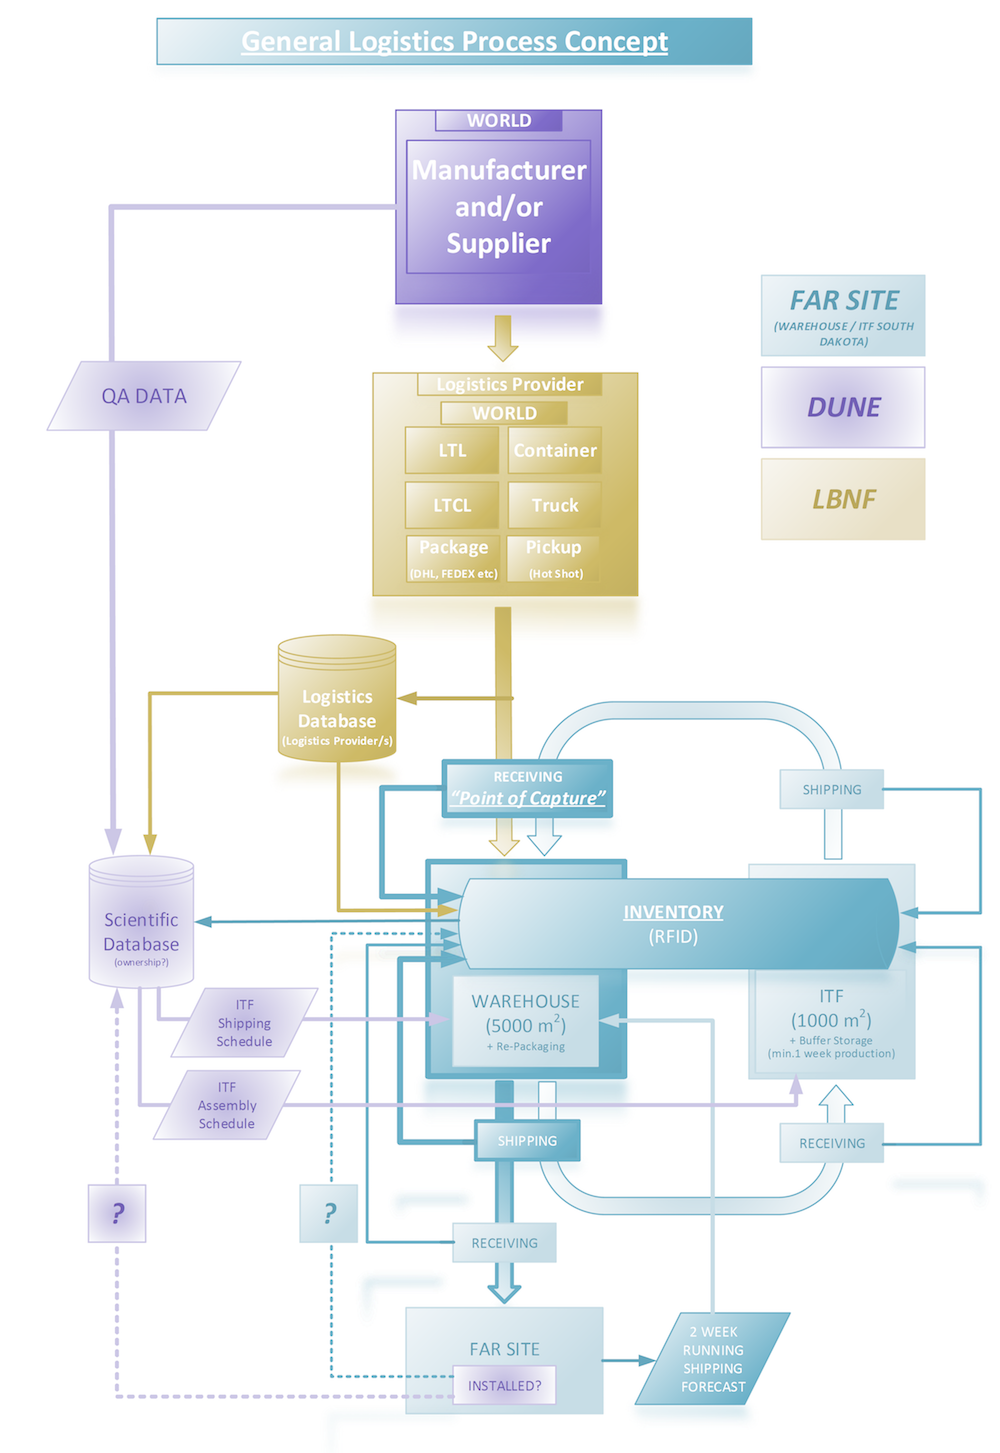
\includegraphics[width=0.65\textwidth]{logistics.png}
\end{dunefigure}
Everything is inventoried and entered into the hardware database at
the \dword{lc} and the \dword{lc} is responsible for trucking between
the \dword{itf} and \surf and for dunnage coming back. The \dword{tpc}
components that must go to
the \dword{itf} arrive at the \dword{lc}, are logged into the
inventory system and transported to the \dword{itf} as
needed. Once the integration is complete, \dword{apa} pairs are
transported back to the \dword{lc} ready to be shipped underground.
The team of riggers and equipment operators are trained professionals
that move all the \dword{tpc} components and infrastructure but also
are trained to assist as needed with integration. The organization of
the \dword{lc} and \dword{itf} are shown in
Figure~\ref{fig:orgchart_itf}.
\begin{dunefigure}[Org Chart for the \dword{lc} and \dword{itf}.]{fig:orgchart_itf}
  {Organization chart for the \dword{lc} and \dword{itf}.}
  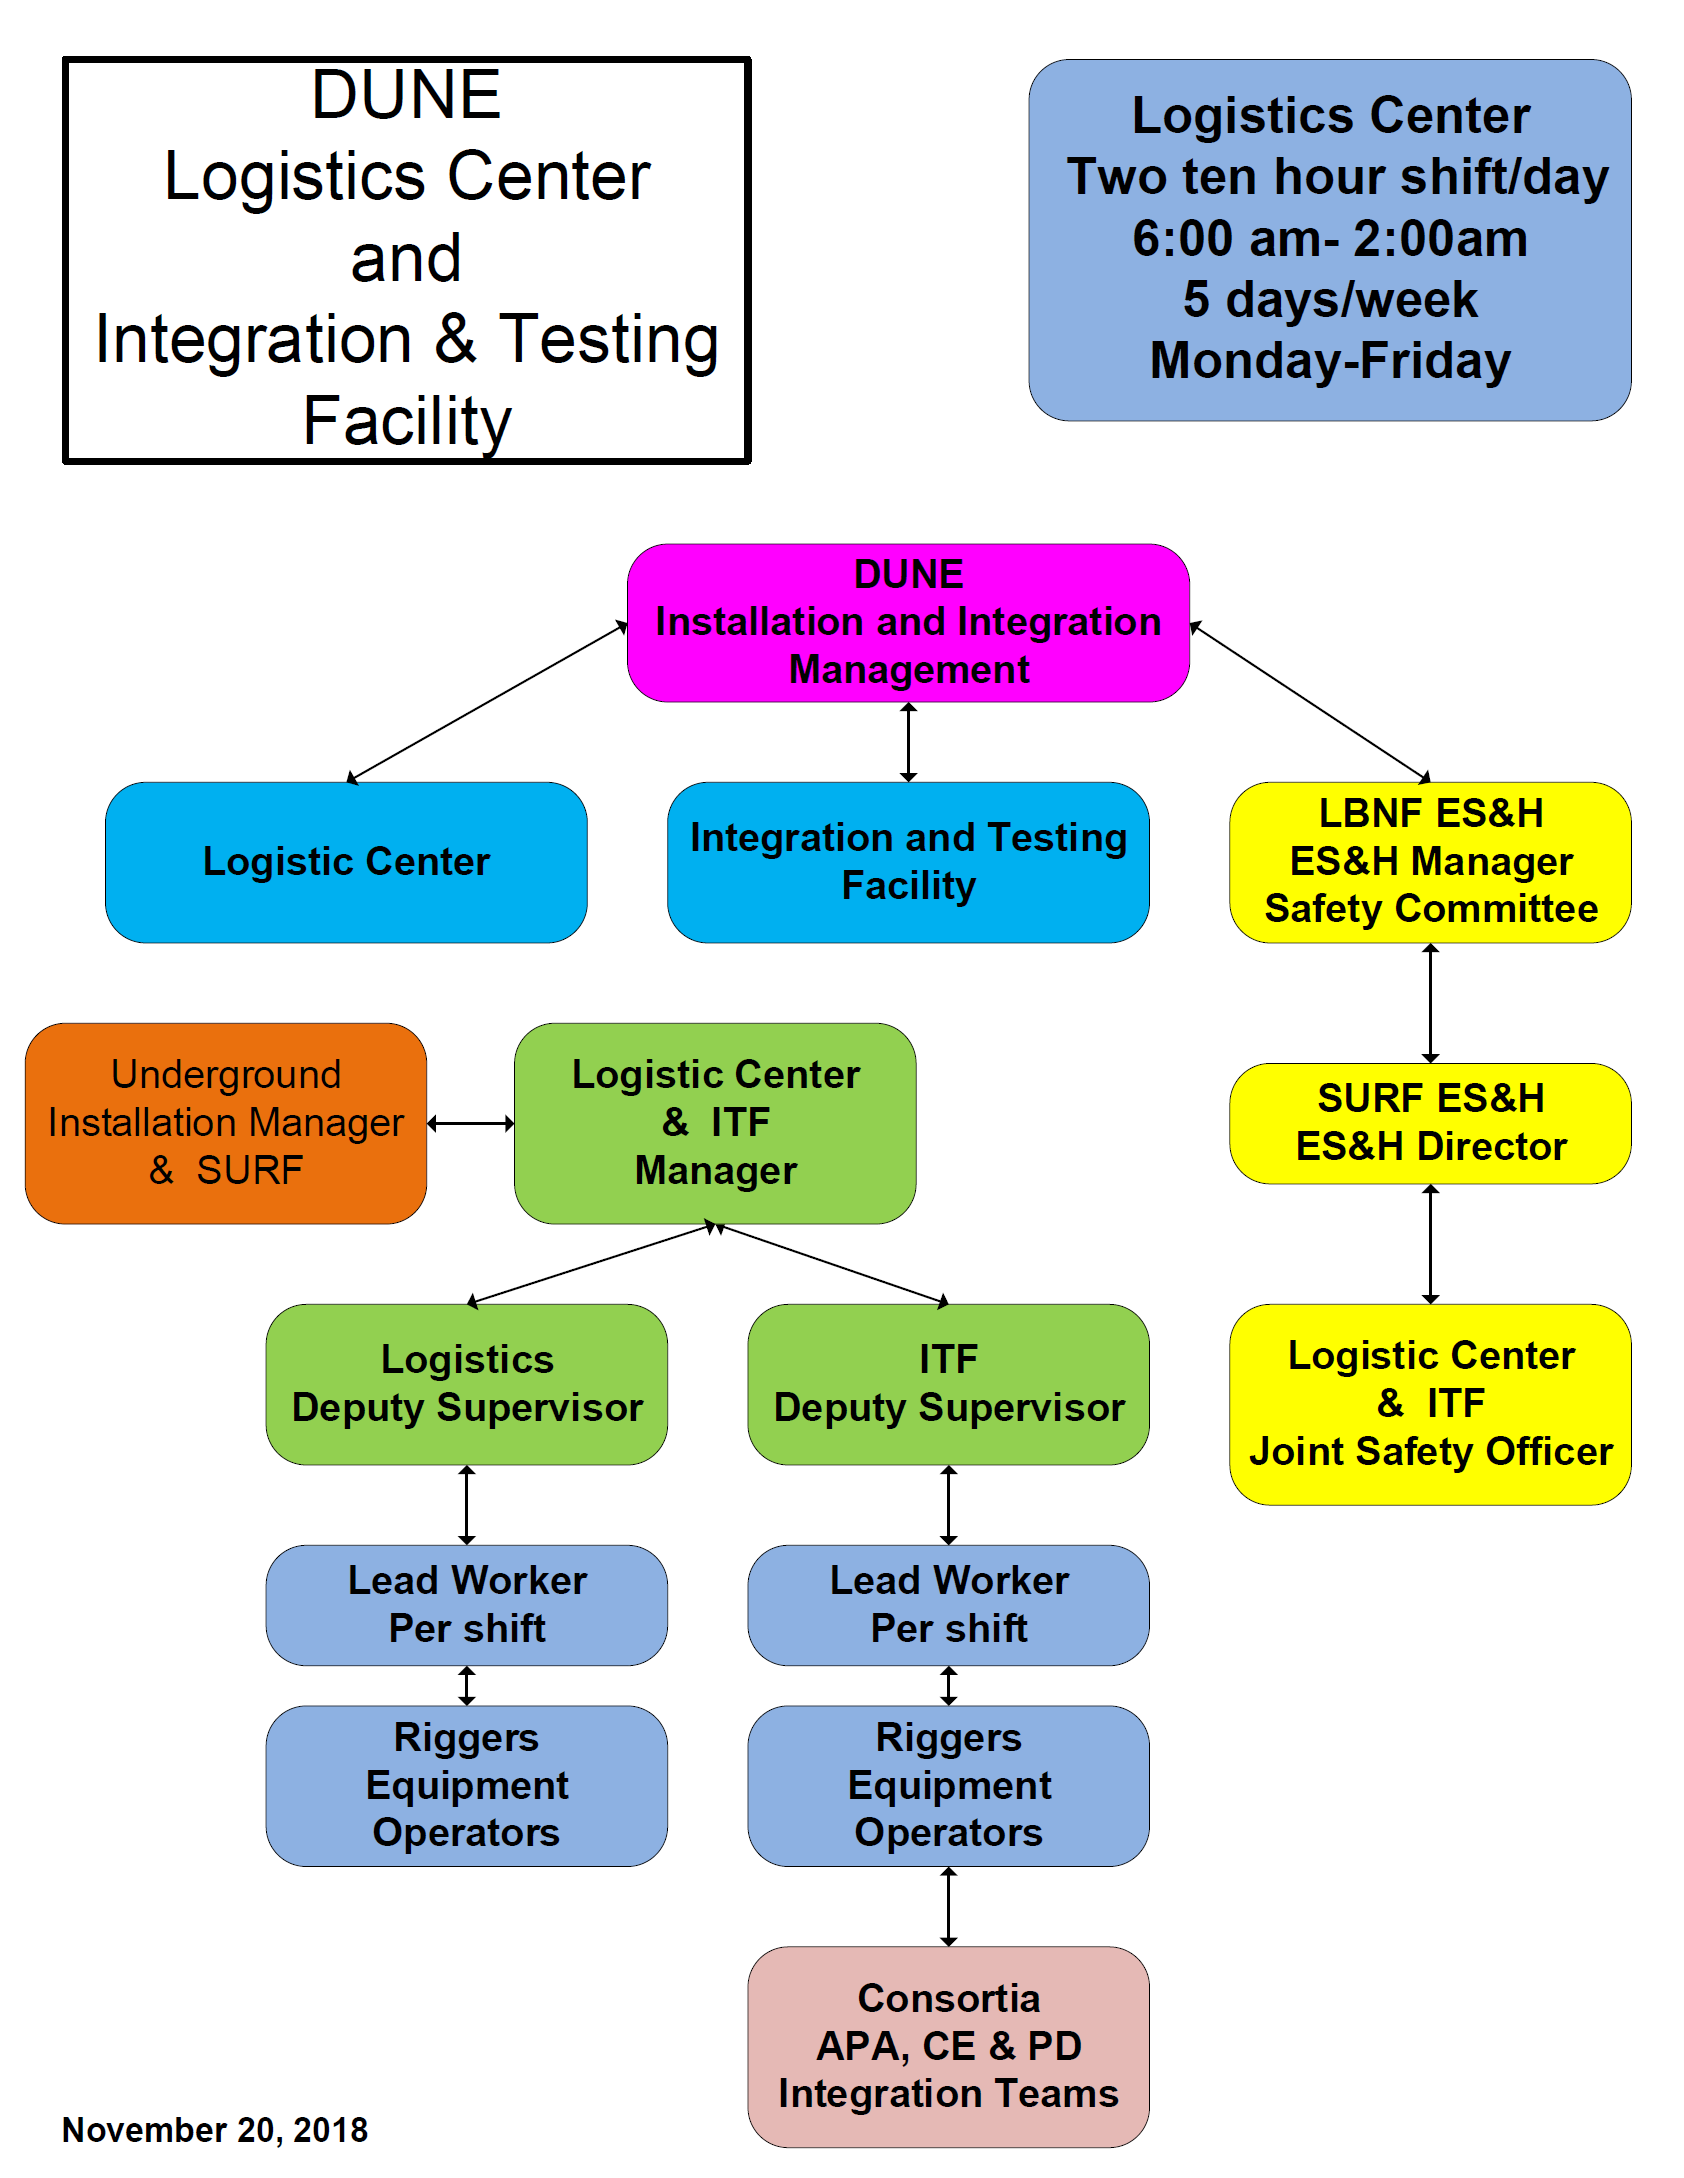
\includegraphics[width=0.65\textwidth]{lc.png}
\end{dunefigure}

\subsubsection{\dword{lc}}

The \dword{lc} is a shipping and handling facility with a smaller crew
than \dword{itf}, but it must operate 20 hours a day, 5 days a week.
This will require 2 rigging/operator crews that will be managed by a
joint management team working in concert with the \dword{itf} that
includes a manager, two deputy supervisors (from the \dword{lc} and
\dword{itf}), an administrative assistant, and a safety officer
working under the direction of Fermilab Safety.  Each shift would have
a lead worker who directs the crew of $\sim$5 \dword{fte} responsible for the
rigging and equipment operation for the shipping and receiving.  Their
tasks would also include using the inventory system to track all
materials coming in and out of the \dword{lc}. Some repackaging will
be required to fit materials in the cage or on a slung load.
Management must work directly with the \dword{lbnf} logistics team at
\surf and \dword{cmgc} so that loads to the headframe arrive as
scheduled.  The headframe has room for only 1 or 2 trucks, so proper
scheduling is critical.

\subsubsection{Integration and Test Facility (ITF)}

The \dword{itf} is where the integration of the
\dword{apa}, \dword{ce}, and \dword{pds} are completed. While the
consortia does most of this technical work and testing, a team of
riggers and equipment operators move the \dword{apa}s on
and off the trucks and around the cleanroom.  The \dword{apa}s are
built at a rate that means the \dword{itf} must start integration
approximately 2 years before the detector is assembled.  This will
also serve as a training period for \dword{uit} staff as things start
to progress underground.  The estimated work force at the \dword{itf} is a
deputy supervisor, a lead worker, and a crew of 3--4 riggers and
equipment operators.  This crew helps as needed with the
integration of the \dwords{apa} to minimize wasted time.

The \dword{lc} and \dword{itf} management work directly with the
consortia to ensure that components are available when
needed using the inventory system.
  

\subsection{Underground Facilities}

\surf/\dword{cmgc} will move \dword{tpc} materials from the
ROss headframe to the caverns. From the cavern entrance, the materials are
handled by the \dword{uit}. The responsibilities of the \dword{uit} are
more complex because of the material movement involved:
\begin{itemize}
 \item North, Central and South Caverns: \dword{tpc} components and
   infrastructure materials can be stored in the available cavern
   space during the construction of detectors \#1--2.  The \dword{uit} team will
   use forklifts, carts and cavern crane to move
   materials into the clean room.
 \item Inside the \dword{sas} and clean room: The main tasks are manipulating \dwords{apa}
   onto the different \dword{apa} towers and \dword{cpa} component
   assembly.  The team operates the shuttle beam and crane, opens and closes the
   cold boxes and moves materials with forklift, carts and motorized
   pallet jacks.
 \item Inside the Cryostat: The \dword{uit} team installs the \dword{dss} and detector
   subfloor; they then move the completed \dword{apa} and \dword{cpa} pairs into
   position.  They also deploy the \dword{fc}.
\end{itemize}

These teams work four 10-hour day and afternoon shifts.  Depending on
available cage trips for shift movement, lead workers,
safety officer and management would have overlapping shifts to insure 
proper transfer of knowledge.  Typically, this would happen at the daily
toolbox safety meeting and work assignment updates.  The safety
officer on each shift would be responsible for any discussion of safety
during the meeting but also for training all workers, including those from
the consortia. The safety officer management goes directly to the \surf
and \dword{lbnf} \dword{esh} to minimize any conflict of interest although 
all \dword{uit} and consortia personnel have the right to stop
work for any safety issues.

\subsubsection{Underground Facilities Management}

Figure~\ref{fig:orgchart_uit} shows management of the \dword{uit}. 
\begin{dunefigure}[Org Chart for the \dword{uit}.]{fig:orgchart_uit}
  {Organization chart for \dword{dune} \dword{uit}.}
  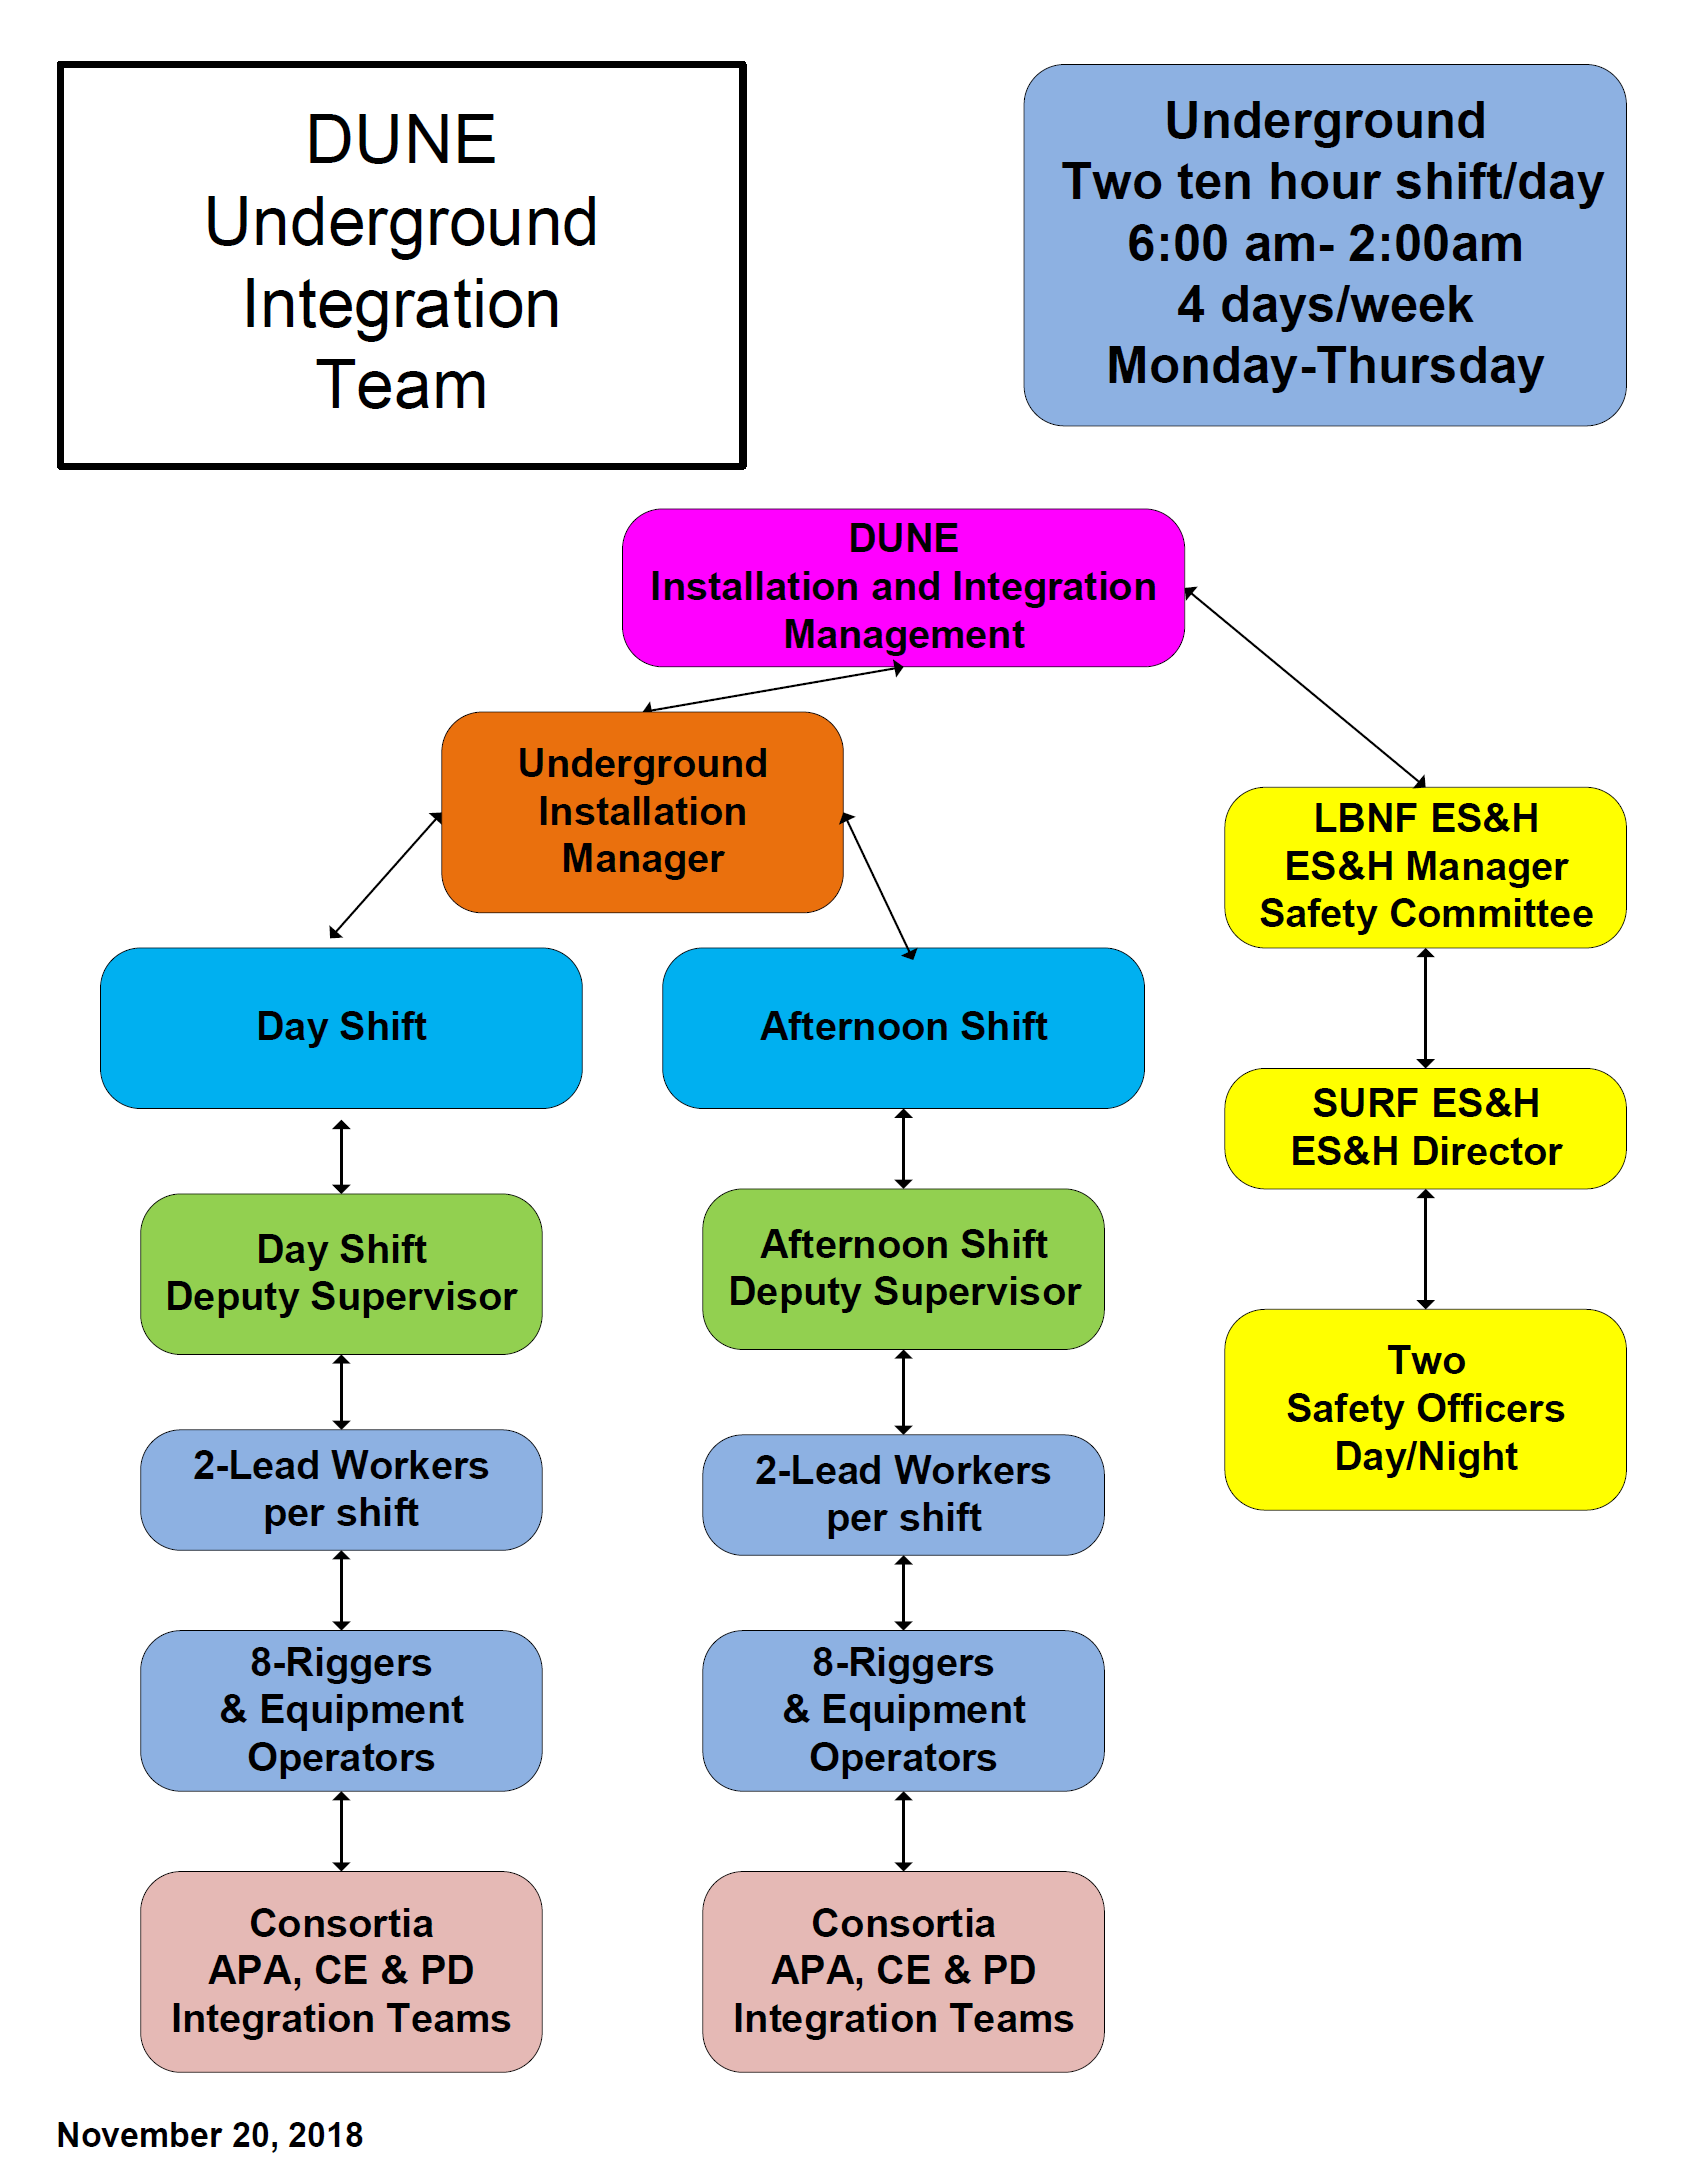
\includegraphics[width=0.5\textwidth]{uit.png}
\end{dunefigure}
\dword{uit}and consists of three levels:
\begin{itemize}
  \item Underground Installation Manager: The \dword{uit} manager oversees
    both shifts but also covers for the day or night shift deputy
    manager if needed.  This manager is the contact person working directly
    with the logistics manager and \surf/\dword{cmgc} to organize cage
    trips for materials needed underground, attending all high-level
    meetings as required, and submitting weekly reports.  The \dword{uit} manager schedules and
    organizes the work along with the consortia to ensure they have
    the rigging crews at the appropriate times.
  \item Day/Night Deputy Installation Supervisors: The deputy
      supervisors are working managers, trained
      riggers and equipment operators who can fill in as needed.  They
      are trained in all installation procedures, working
      directly with the consortia to keep the project 
      on schedule.  If the lead worker is sick or on vacation, the deputy supervisors fill in. Communication among the deputy supervisors between
      shifts is critical for a smooth shift change.
  \item Lead Workers: The lead workers typically are the main
    equipment operators and direct the individual teams, which typically comprise 2 or 3
    riggers or equipment operators.  The lead workers are trained in all
    installation procedures and help the consortia as needed for
    each task.  Two lead workers per shift shift as
    needed between the main cavern, materials \dword{sas}, clean room, and
    inside and on top of the cryostat.
  \item Riggers and Equipment Operators: Riggers and equipment
    operators are trained in both roles; they
    can run the cranes, forklifts, and other equipment as needed.  They
    work in two person teams at a minimum, more if a
    task requires it. Typical \dword{apa} movement requires at least three workers and a
    spotter. They are also well trained in all installation
    procedures and can help as needed.
\end{itemize}

\subsection{Ash River}

Ash River is the site of the NOvA far detector in Ash River,
Minnesota. The NOvA far site detector hall offers a \SI{16.75}{m} deep
pit with $\sim$\SI{300}{m$^2$} of floor space available for testing
DUNE detector components at full scale.  The trial assembly work at
Ash River has three major phases of \dword{dune} mechanical tests to
confirm designs and practice installation techniques, particularly if
the design has been modified from \dword{protodune}.  The \dword{nova}
Far Detector Laboratory is managed by the University of Minnesota and
is partially funded through an operations grant from Fermilab.  We follow both
university and Fermilab safety regulations, whichever is more
stringent.  The university code officials approve all building
permits, which include engineered drawings signed by an engineer
registered in Minnesota. All hazard analyses and work procedure
documents are approved by a joint safety committee with members drawn
from both the University of Minnesota and Fermilab and may include
specialists as needed.

The work at Ash River has three main goals: verify that the
\dword{dune} \dword{tpc} can be installed as safely and efficiently as
possible; complete a set of procedural documents as the basis of
documentation for work underground; and serve as a training center for
new hires at \surf so underground procedures are well understood.

There is a full time staff of five \dwords{fte} at Ash River. A manager,
deputy manager and 3 experienced technicians.  One of the technicians
is also our safety officer and is the chairperson of the joint safety
committee.


Phase 0: This work has started now.  A vertical cable test of two
full-scale \dword{apa} side tubes have been mounted to a column in the
lab. Using a complete cable bundle we will test how well the conduit
system works and possible modifications. We have
completed a series of schemes for mounting the \dword{gp}
on the \dword{fc}.

Phase 1: We will construct a prototype of the \dword{dune} \dword{apa}
tower using a steel frame large enough to hold a commercial stair
scaffold in the middle as can be seen in Figure ~\ref{fig:ashriver1}.
\begin{dunefigure}[View of the Ash River Phase 1 assembly.]{fig:ashriver1}
  {Phase 1 Trial Assembly \dword{apa} Tower at the NOvA Far Detector
    Lab in Ash River.}
  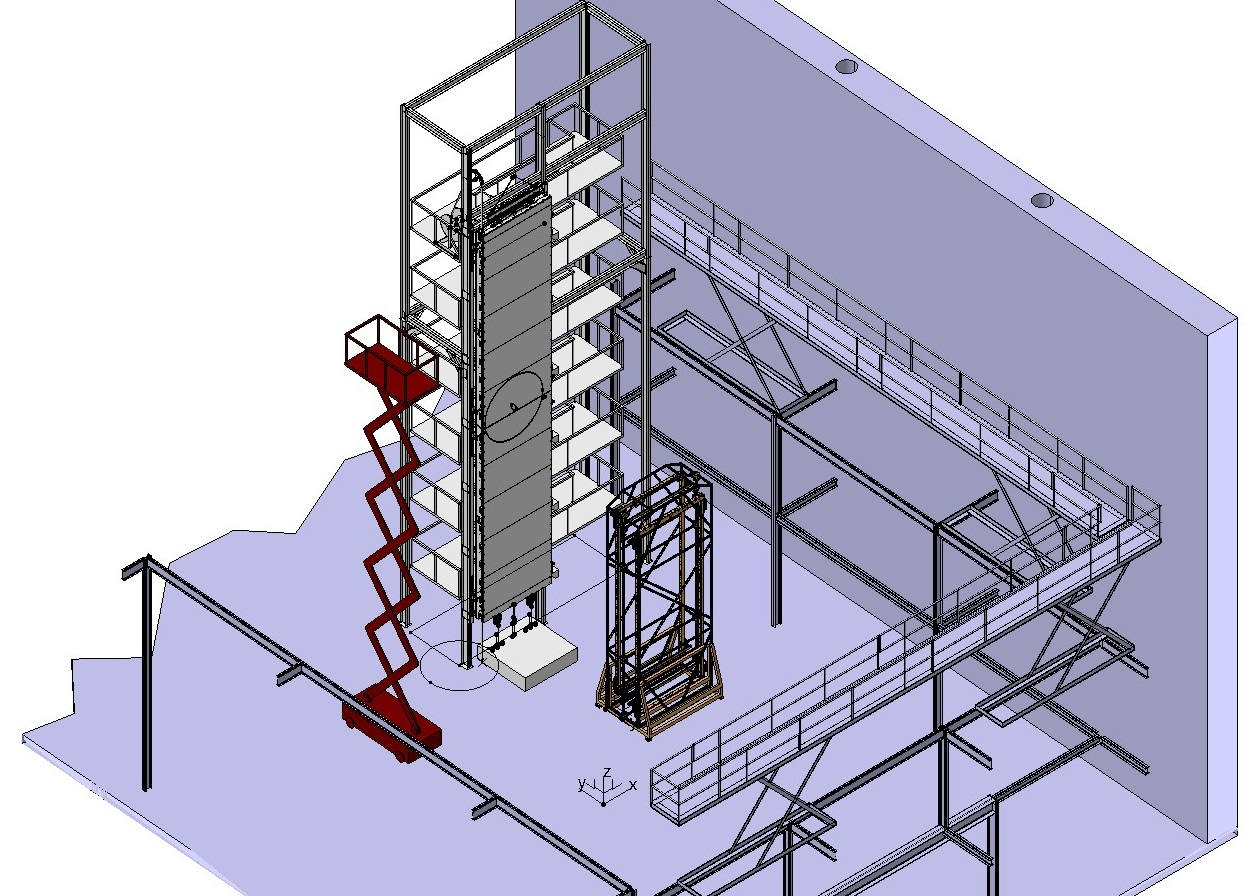
\includegraphics[width=0.65\textwidth]{phase1.jpg}
\end{dunefigure}
This \dword{apa} tower will be designed so we can
use it for joining the top and bottom \dword{apa}s together and all the
cabling. Procedures for removing the cable conduits and replacing
failed Photon Detectors will also be developed.

Phase 2: A more complex structure which mocks up the shuttle
beam/crane in the cleanroom will be needed. A schematic can be seen in
Figure~\ref{fig:ashriver2}.
\begin{dunefigure}[View of the cleanroom for the \dword{dsp} detector
    \#1 showing the shuttle beam system]{fig:ashriver2}
  {View of the cleanroom for the \dword{dsp} detector \#1 showing the
    shuttle beam system}
  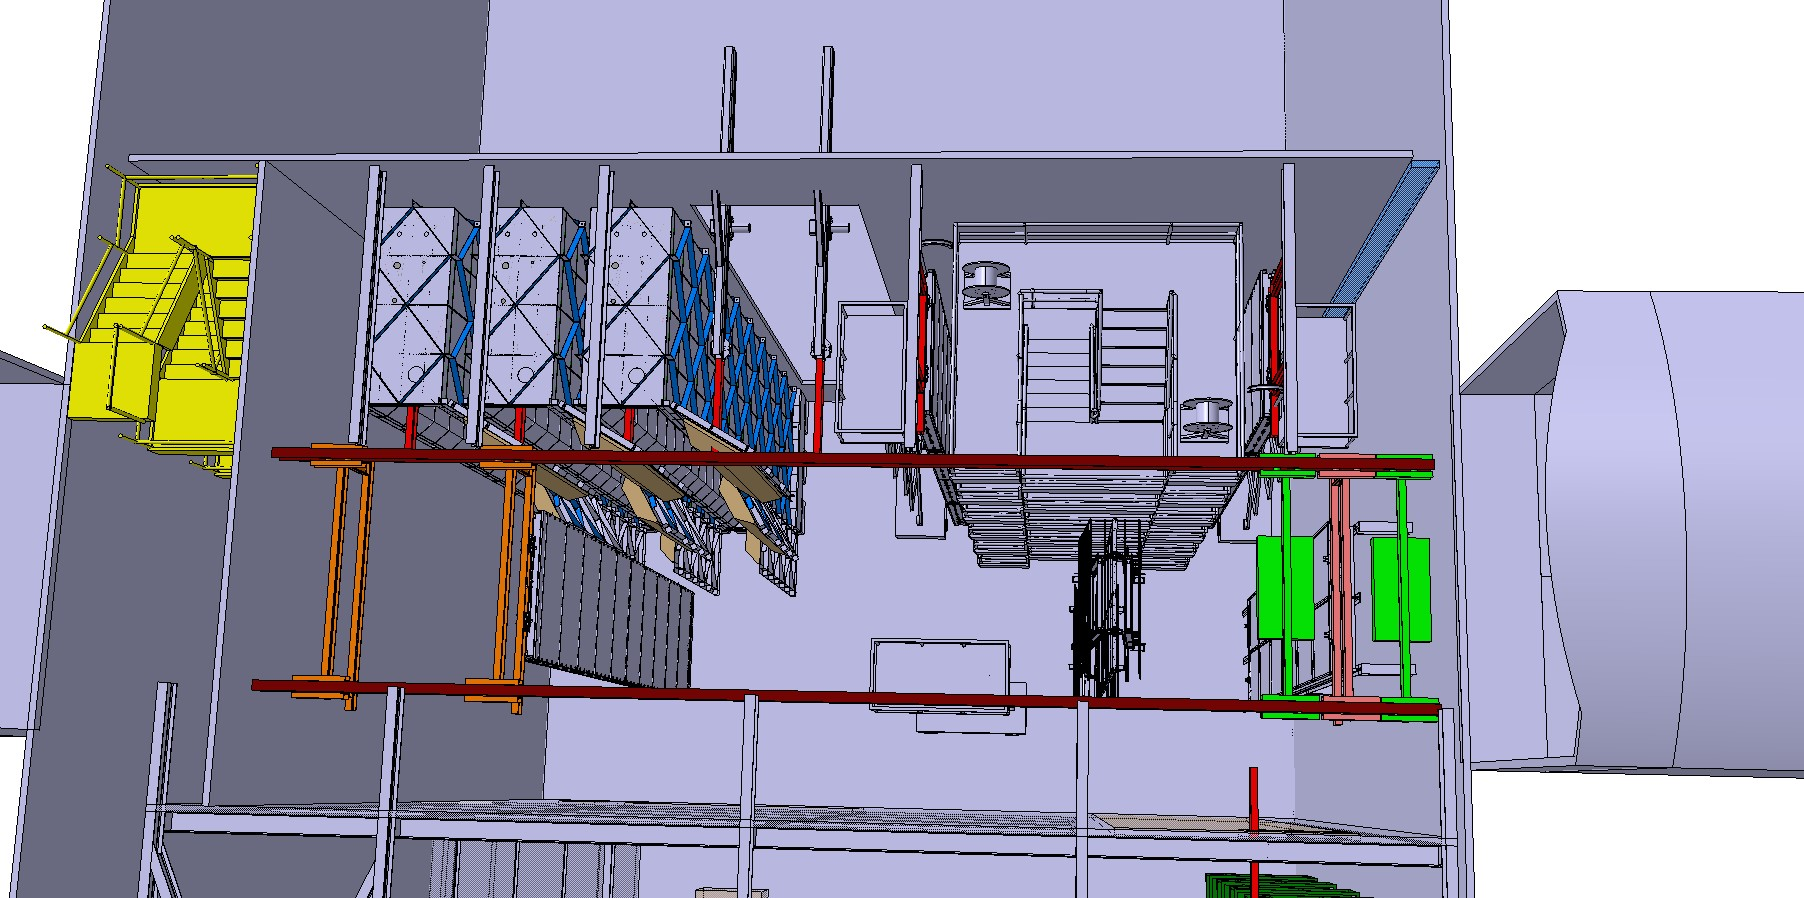
\includegraphics[width=0.65\textwidth]{phase2.jpg}
\end{dunefigure}
This is a very similar to the existing design of the shuttle beam in
the cryostat.  As we proceed with the phase 1 tests, we will adapt the
cleanroom rail system or cryostat rail system to allow full movement
of the \dword{apa} and \dword{cpa} pairs. We would decide how best to
allow us to do a full-scale test of the rest of the installation
procedures using this structure including:
\begin{itemize}
 \item Installation of the Detector Support System (DSS)
 \item Transfer of TPC component through the TCO
 \item Moving \dword{apa} and \dword{cpa} pairs into ``final'' position and deploying the field cages
 \item Cabling of the \dword{apa} through the cryostat penetrations
 \item Installation of the end walls
 \item Potentially deployment of the Dual Phase detector
\end{itemize}

\section{\dword{dune} Host Facility Services}
\label{sec:fdsp-coord-host_facility_services}

This section is under development. The plan is to ask Patrick to write
it.

The intent of this section is to describe the services that are
provided by the host facility.

The following is preliminary outline, there may already be a document
with a more comprehensive plan.
\begin{itemize}
\item Detector component transportation to underground cavern and rigging
\item Removal of equipment packaging from undergoing cavern
\item Electical and plumbing contracted services
\item Maintenance and readiness of lifts, moving equipment and associated items
\item Maintenance and operation of cooling water systems for detector and CUC
\item Maintenance and operation of networking equipment
\item Maintenance and operation of electrical installations for detector power
\item Building and cavern services such as lighting, air handling and
  filtration, fire safety and suppression, safety rails, dew point
  control, hazard alarms (fire and ODH)
\item Hazard awareness and safety training
\item Storage areas for tools and PPE
\item Facility life saftey systems
\item Plan for medical emergencies and medical evacuation
\item Underground emergency plans and procedures
\item Controlled access plan and equipment
\item Maintenance of ground impedance monitors and detector ground Isolation
\end{itemize}


